\documentclass[pmlr]{jmlr}% PMLR format (Deep Learning Indaba / JMLR-PMLR guidelines)
% jmlr auto-loads: amsmath, amssymb, natbib, graphicx, url, algorithm2e.

\usepackage{booktabs}
\usepackage{xurl}% allow long URLs to break across lines
\usepackage{float}
\usepackage{tcolorbox}
\usepackage{tikz}
\usetikzlibrary{positioning,shapes.geometric,arrows.meta,calc}
\graphicspath{{figures/}}
\newcommand{\acc}{\mathrm{Acc}}

\jmlrvolume{}
\jmlryear{2026}
\jmlrworkshop{Trustworthy AI Workshop, Deep Learning Indaba 2026}

% Remove the first-page copyright footer, and the running header on pages 2+.
\makeatletter
\renewcommand*{\@titlefoot}{}
\makeatother

\title[Confidently Wrong: Calibration Risks in LLMs for African Languages]{Confidently Wrong: Measuring and Mitigating Calibration Risks in LLMs for African Languages}

\author{%
  \Name{Similoluwa Okunowo} \Email{similoluwa@aims.ac.za}\\
  \Name{Eliud Koto} \Email{eliud@aims.ac.za}\\
  \Name{Dagmawi Misker} \Email{dagmawi@aims.ac.za}\\
  \addr African Institute for Mathematical Sciences (AIMS), South Africa
}

\begin{document}

\maketitle
\thispagestyle{jmlrtps}% keep the PMLR line on page 1
\pagestyle{plain}% no running header on pages 2+ (page numbers only)
\vspace{-2.2em}% tighten the gap between authors and abstract

\begin{abstract}
Large language models (LLMs) are increasingly used in African languages, yet little is known about
whether their confidence remains reliable. This creates a safety risk: models may become less
accurate while remaining highly confident, increasing the likelihood of trusted misinformation. We
evaluate four open-weight LLMs (\textbf{Qwen3-4B-Instruct}, \textbf{Gemma-4-12B},
\textbf{Aya-Expanse-8B}, and \textbf{AfroLlama-V1}) on African-language truthfulness and knowledge
benchmarks (\textbf{Uhura-TruthfulQA} and \textbf{AfriMMLU}), measuring calibration using
log-probability-based confidence estimates. We find that most models are systematically more
overconfident on African languages than on English (the Africa-adapted AfroLlama-V1 is a partial
exception), often placing high confidence on incorrect answers and producing a marked increase in
expected calibration error. Among three mitigation
strategies, temperature scaling proves most effective, reducing calibration error substantially
without retraining. Our findings suggest that African-language deployment risks stem not only
from lower accuracy but also from models remaining confident when wrong, and that simple post-hoc
recalibration offers a practical deployment-time safety intervention.
\end{abstract}

\section{Introduction}
LLMs are entering high-stakes, information-seeking use in African languages, in domains such as
health, legal, educational, and civic information, often where users cannot easily verify an answer. The safety
failure we study is a mismatch between confidence and correctness. When models remain highly
confident despite being wrong, they can mislead users into treating incorrect information as
reliable, which is particularly dangerous in high-stakes settings such as health, education, and
civic information. A calibrated model, whose confidence tracks its accuracy, can instead
\emph{abstain}, declining or deferring when uncertain \citep{tomani2024}. If calibration holds in
English but breaks in African languages, the populations least served by current models are most
exposed to confident misinformation. We investigate whether models become increasingly overconfident
in African languages, quantify the extent of this misalignment between confidence and correctness,
and evaluate practical strategies for mitigating it.

\medskip
\noindent\textbf{Our main contributions are:}
\begin{enumerate}\itemsep1pt
  \item An open-weight, reproducible calibration audit of four LLMs on African-language truthfulness
  and knowledge benchmarks, using answer-text log-probabilities to obtain robust confidence estimates
  for instruction-tuned models.

  \item Evidence that calibration degrades substantially from English to African languages, revealing
  systematic overconfidence and a growing mismatch between confidence and correctness across models
  and tasks.

  \item An evaluation of practical mitigation strategies, including temperature scaling, abstention,
  and few-shot prompting, together with a deployment framework showing that lightweight post-hoc
  recalibration is an effective safety intervention for African-language LLMs.
\end{enumerate}

\section{Related Work}
Neural networks are often overconfident, and temperature scaling is a standard single-parameter
post-hoc calibration method \citep{guo2017}; for free-form generation, sampling-based methods such as
semantic entropy estimate uncertainty without labelled data \citep{kuhn2023}. \citet{tomani2024}
show that uncertainty-based abstention improves correctness, reduces hallucinations, and increases
safety, motivating uncertainty estimation as a deployment-time safety mechanism. African-language
evaluation has advanced through human-translated benchmarks, including Uhura for truthfulness and
scientific question answering \citep{uhura} and AfriMMLU within IrokoBench for knowledge evaluation
\citep{irokobench}, alongside models such as AfroLlama \citep{afrollama}. However, prior work has
focused primarily on capability and benchmark performance. To our knowledge, calibration in African
languages, compared across models and paired with mitigation strategies, has not been systematically
studied.

\section{Methods}

\subsection{Models}
We evaluate four open-weight models chosen to span size, multilinguality, and origin: a small
instruction-tuned model, a larger one, a multilingual one, and an Africa-specific one (full
specifications in Table~\ref{tab:models}, Appendix~\ref{app:models}). Open weights give direct
log-probability access and full reproducibility without proprietary APIs.

\subsection{Datasets}
We use Uhura-TruthfulQA \citep{uhura} (English and six African languages; truthfulness; a variable
number of candidate answers per question) and AfriMMLU \citep{irokobench} (18 languages; knowledge;
four options per question). Because their language sets and tasks differ, we analyse them separately
and never average across them. ``African'' denotes all languages other than English and French.

\subsection{Scoring}
For both datasets we score each option by the length-normalised log-probability of its answer text
(a cloze reading; Appendix~\ref{app:scoring}) and take the softmax over options as the model's
confidence. We deliberately avoid letter-logit scoring (reading the next-token probability of
``A''/``B''/``C''/``D''): it silently collapses instruction-tuned models, with Gemma-4-12B returning
``A'' for 75\% of items and scoring below chance, whereas answer-text scoring did not collapse for any model.

\subsection{Metrics}
We report expected calibration error (ECE, 15 bins), overconfidence (mean confidence minus accuracy),
Brier score, error-detection AUROC, and AUARC, the area under the accuracy-rejection curve
(definitions in Appendix~\ref{app:metrics}).

\subsection{Interventions}
We evaluate three: per-language temperature scaling, selective abstention by per-language confidence
threshold, and 5-shot in-context prompting with examples held out from evaluation
(Appendix~\ref{app:interventions}).

\section{Results}\label{sec:results}
Table~\ref{tab:overview} summarises every model on both datasets; the central finding is the gap
between English and African-language calibration.

\begin{table}[t]\centering\small
\caption{English versus African-language performance, by model and dataset. ``en'' is English and
``afr'' is the mean over African languages; ECE(TS) is pooled ECE after per-language temperature
scaling; AUARC measures abstention quality (higher is better). Models are accurate and calibrated in
English but lose both in African languages, and recalibration restores calibration.}
\label{tab:overview}
\resizebox{\textwidth}{!}{%
\begin{tabular}{llcccccc}
\toprule
\textbf{Model} & \textbf{Dataset} & \textbf{Acc(en)} & \textbf{Acc(afr)} & \textbf{ECE(en)} & \textbf{ECE(afr)} & \textbf{ECE(TS)} & \textbf{AUARC}\\
\midrule
Qwen3-4B-Instruct & Uhura-TruthfulQA & 0.38 & 0.32 & 0.07 & 0.17 & \textbf{0.03} & 0.36\\
Gemma-4-12B       & Uhura-TruthfulQA & 0.33 & 0.34 & 0.21 & 0.26 & \textbf{0.03} & 0.39\\
Aya-Expanse-8B    & Uhura-TruthfulQA & 0.36 & 0.31 & 0.08 & 0.20 & \textbf{0.04} & 0.35\\
AfroLlama-V1      & Uhura-TruthfulQA & 0.29 & 0.33 & 0.18 & 0.13 & \textbf{0.04} & 0.35\\
\midrule
Qwen3-4B-Instruct & AfriMMLU & 0.53 & 0.30 & 0.06 & 0.15 & \textbf{0.02} & 0.35\\
Gemma-4-12B       & AfriMMLU & 0.30 & 0.27 & 0.31 & 0.34 & \textbf{0.07} & 0.29\\
Aya-Expanse-8B    & AfriMMLU & 0.52 & 0.29 & 0.06 & 0.18 & \textbf{0.02} & 0.34\\
AfroLlama-V1      & AfriMMLU & 0.36 & 0.28 & 0.22 & 0.20 & \textbf{0.03} & 0.31\\
\bottomrule
\end{tabular}}
\end{table}

\begin{enumerate}\itemsep2pt
  \item \textbf{Calibration degrades from English to African languages for most models.} For the three
  general-purpose models, ECE and overconfidence are substantially higher in African languages
  (Table~\ref{tab:overview}, Figure~\ref{fig:calib}); in aggregate, models are most overconfident
  where they are least accurate. AfroLlama-V1, adapted to several of these languages, is the exception:
  its African ECE is no higher than its English ECE on both datasets (Appendix~\ref{app:bootstrap}).
  \item \textbf{The accuracy collapse is a knowledge story.} On AfriMMLU the capable models fall from
  about 0.52 (English) to about 0.29 (African, near the 0.25 chance floor). On Uhura, accuracy is
  uniformly low (about 0.31) with little English advantage, so Uhura supplies the calibration signal
  and AfriMMLU the accuracy decay.
  \item \textbf{Mitigations are unequal.} Per-language temperature scaling cuts pooled ECE to about
  0.02 to 0.08 for every model (Appendix Figure~\ref{fig:tempscale}); the fitted temperatures are
  almost always $T>1$ (softening overconfident predictions), and for African languages the optimum is
  typically driven to the top of our grid ($T=5$), showing how far confidence must be discounted.
  Abstention helps less, because
  uncertainty is a weak error-ranker (AUROC about 0.55), so AUARC sits only modestly above baseline.
  Few-shot prompting gives small gains for three models and backfires on Gemma (Appendix
  Table~\ref{tab:fewshot}).
  \item \textbf{Scale alone did not improve calibration.} The largest model we evaluate, Gemma-4-12B,
  is also the worst-calibrated (pooled ECE up to 0.34) and overconfident across every topic. Because
  our models top out at 12B parameters, we make no claim about frontier-scale systems; within this
  range, size offered no calibration benefit.
\end{enumerate}

Per-language bootstrap 95\% confidence intervals are reported in Appendix~\ref{app:bootstrap}
(Table~\ref{tab:bootstrap_ci}).

\begin{figure}[t]\centering
  \begin{minipage}{0.49\textwidth}\centering
    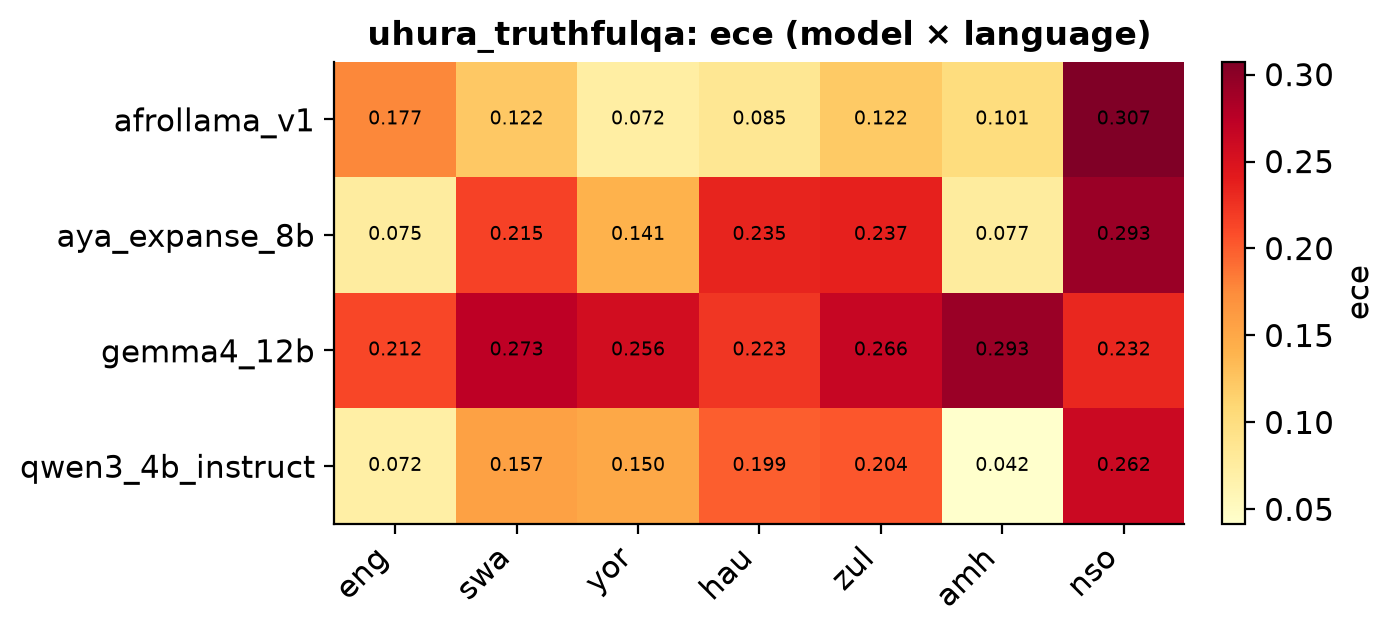
\includegraphics[width=\linewidth]{uhura_ece_heatmap.png}\\[2pt]{\small (a) Uhura-TruthfulQA (7 languages)}
  \end{minipage}\hfill
  \begin{minipage}{0.49\textwidth}\centering
    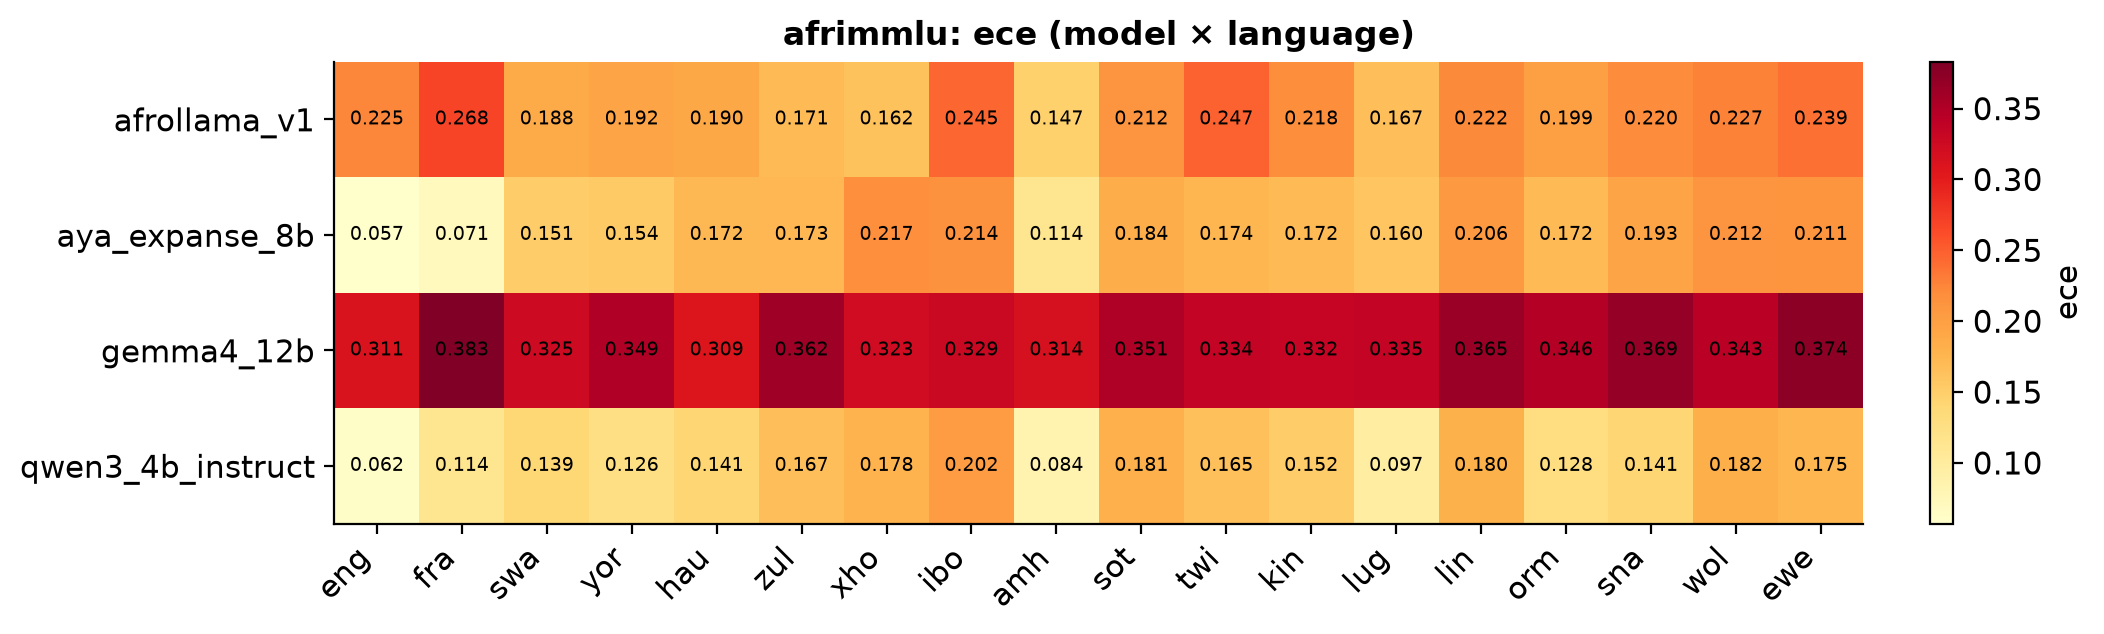
\includegraphics[width=\linewidth]{afrimmlu_ece_heatmap.png}\\[2pt]{\small (b) AfriMMLU (18 languages)}
  \end{minipage}
  \caption{Expected calibration error by model and language. For most models ECE is low in English and
  French and increases for African languages; Gemma-4-12B is an outlier, poorly calibrated even in
  English and the worst-calibrated overall. The pattern holds under answer-text scoring, not as a
  letter-logit artifact.}
  \label{fig:calib}
\end{figure}

\section{Discussion and Limitations}
\textbf{Implications for African AI safety.} In African languages these models are at once less
accurate and more overconfident, the worst combination for trust, since confident wrong answers
reach users precisely where verification is hardest (Appendix~\ref{app:examples} gives concrete
examples). Encouragingly, much of the failure is an
output-layer problem: cheap, post-hoc, per-language temperature scaling closes most of the
calibration gap with no retraining, so safer deployment is feasible now, and it needs only a small
in-language calibration set (about 25 to 50 items per language; Appendix~\ref{app:sensitivity}). Abstention alone is
insufficient because the uncertainty signal is weak, so the durable fix remains better
African-language data and training. We distil this into a deployment framework
(Appendix~\ref{app:framework}): recalibrate, then route on calibrated confidence to answer, ask for
more context, or abstain, logging low-confidence queries for data collection.

\textbf{Limitations.} Accuracies are near chance on these hard, low-resource tasks, so we document
systematic overconfidence rather than catastrophic confident-wrongness, and absolute ECE is moderate
except for Gemma. The weak uncertainty signal (AUROC about 0.55) bounds how much abstention can help.
We cover four open models and two benchmarks; reasoning and frontier closed models were out of scope.

\textbf{Future work.} Extending the audit to reasoning and closed frontier models; in-context
calibration at scale; the offline data-collection loop in Figure~\ref{fig:framework}; and
human-grounded evaluation of abstention.

\section{Conclusion}
Open LLMs are confidently wrong in African languages: for most models, less accurate and more
overconfident than in English across both tasks. Post-hoc per-language temperature scaling is a cheap,
effective safety lever that closes most of the calibration gap, and our deployment framework pairs it
with thresholded abstention for safer real-world use.

\acks{We thank Apart Research for organising the Global South AI Safety Hackathon, which motivated and
supported this work.}

\begin{thebibliography}{9}\small
\bibitem[Guo et al.(2017)]{guo2017} Guo, C., Pleiss, G., Sun, Y., and Weinberger, K. Q. (2017). On
Calibration of Modern Neural Networks. \textit{Proceedings of the 34th International Conference on
Machine Learning (ICML)}, PMLR 70:1321--1330. arXiv:1706.04599.
\bibitem[Kuhn et al.(2023)]{kuhn2023} Kuhn, L., Gal, Y., and Farquhar, S. (2023). Semantic
Uncertainty: Linguistic Invariances for Uncertainty Estimation in Natural Language Generation.
\textit{International Conference on Learning Representations (ICLR)}. arXiv:2302.09664.
\bibitem[Tomani et al.(2024)]{tomani2024} Tomani, C., Chaudhuri, K., Evtimov, I., Cremers, D., and
Ibrahim, M. (2024). Uncertainty-Based Abstention in LLMs Improves Safety and Reduces Hallucinations.
arXiv:2404.10960.
\bibitem[Bayes et al.(2024)]{uhura} Bayes, E., Azime, I. A., Alabi, J. O., Kgomo, J., Eloundou, T.,
Proehl, E., Chen, K., Khadir, I., Etori, N. A., Muhammad, S. H., Mpanza, C., Thete, I. P., Klakow, D.,
and Adelani, D. I. (2024). Uhura: A Benchmark for Evaluating Scientific Question Answering and
Truthfulness in Low-Resource African Languages. arXiv:2412.00948.
\bibitem[Adelani et al.(2024)]{irokobench} Adelani, D. I., et al. (2024). IrokoBench: A New Benchmark
for African Languages in the Age of Large Language Models. arXiv:2406.03368.
\bibitem[Jacaranda Health(2024)]{afrollama} Jacaranda Health (2024). AfroLlama-V1. Hugging Face.
\url{https://huggingface.co/Jacaranda/AfroLlama_V1}.
\end{thebibliography}

\appendix
\vspace{2.5em}
\noindent{\Large\bfseries Appendix}\par
\vspace{0.6em}

\section{Models}\label{app:models}
\begin{table}[H]\centering\small
\caption{Open-weight models evaluated.}
\label{tab:models}
\resizebox{\textwidth}{!}{%
\begin{tabular}{llll}
\toprule
\textbf{Model} & \textbf{Params} & \textbf{Type} & \textbf{Hugging Face ID}\\
\midrule
Qwen3-4B-Instruct & 4B  & Instruction-tuned & \texttt{Qwen/Qwen3-4B-Instruct}\\
Gemma-4-12B       & 12B & Instruction-tuned & \texttt{google/gemma-4-12b-it}\\
Aya-Expanse-8B    & 8B  & Multilingual      & \texttt{CohereLabs/aya-expanse-8b}\\
AfroLlama-V1      & 7B  & Africa-specific (LLaMA-2 base) & \texttt{Jacaranda/AfroLlama\_V1}\\
\bottomrule
\end{tabular}}
\end{table}

AfroLlama-V1 is based on LLaMA-2-7B and was fine-tuned on Swahili, Zulu, Yoruba, Hausa, Xhosa, and
English; Amharic and N.\,Sotho, which appear in our benchmarks, are out-of-distribution for this
model. All models are loaded in \texttt{bfloat16} with scaled dot-product (\texttt{sdpa}) attention,
a 2048-token context limit, and greedy decoding (temperature 0), on a single NVIDIA A100 (40\,GB).

\section{Metric definitions}\label{app:metrics}
For an item with options $o$ and gold answer $y$, the cloze score of option $o$ with tokens
$o_1,\dots,o_L$ given context $x$ is the length-normalised log-probability
\begin{equation}
s(o) = \frac{1}{L}\sum_{t=1}^{L}\log p(o_t \mid x, o_{<t}).
\end{equation}
\begin{equation}
p(o) = \operatorname{softmax}_o s(o),
\qquad \hat{y}=\arg\max_o p(o), \qquad c=\max_o p(o).
\end{equation}
Over $N$ items with correctness $y_i\in\{0,1\}$, confidence $c_i$, and $B=15$ equal-width confidence
bins $\{B_b\}$:
\begin{equation}
\mathrm{ECE}=\sum_{b=1}^{B}\frac{|B_b|}{N}\,\bigl|\acc(B_b)-\mathrm{conf}(B_b)\bigr| .
\end{equation}
\begin{equation}
\text{Overconfidence}=\frac{1}{N}\sum_i c_i-\frac{1}{N}\sum_i y_i .
\end{equation}
\begin{equation}
\text{Brier}=\frac{1}{N}\sum_i (c_i-y_i)^2 .
\end{equation}
AUROC is the area under the ROC curve using $c$ to rank correct against incorrect items. AUARC is the
area under the accuracy-rejection curve: items are answered most-confident-first and accuracy on the
answered subset is integrated over coverage. Temperature scaling rescales the logits by a single
$T>0$, $p_T(o)=\operatorname{softmax}_o\!\big(s(o)/T\big)$; we fit $T^\star=\arg\min_T \mathrm{ECE}$
on a seeded 50\% calibration split and report ECE on the held-out half.

\section{Prompts}\label{app:scoring}
Each option is scored as a continuation of the prompt; the prompt lists no answer letters.

\begin{tcolorbox}[colback=blue!4,colframe=blue!45,title=\textbf{Uhura-TruthfulQA (truthfulness)},fonttitle=\small,boxrule=0.5pt]
\ttfamily\small Q: \{question\}\\ A:
\end{tcolorbox}

\begin{tcolorbox}[colback=blue!4,colframe=blue!45,title=\textbf{AfriMMLU (knowledge)},fonttitle=\small,boxrule=0.5pt]
\ttfamily\small The following is a multiple-choice question about \{subject\}. Give the correct answer.\\[3pt]
Question: \{question\}\\ Answer:
\end{tcolorbox}

For 5-shot prompting, the prompt is prefixed with five solved examples in the same language, each
formatted as the template above followed by its gold answer text and separated by blank lines; the
examples are held out from evaluation.

\section{Interventions}\label{app:interventions}
By \emph{interventions} we mean lightweight, post-hoc procedures applied at or after inference to
improve calibration or to trade answer coverage for reliability, without any retraining of the model.
We evaluate three:
\begin{enumerate}\itemsep1pt
  \item \textbf{Temperature scaling.} We fit one temperature $T$ per language by minimising ECE on a
  seeded 50\% calibration split and evaluate on the held-out half, searching the grid
  $T \in \{0.5, 0.6, 0.7, 0.8, 0.9, 1.0, 1.2, 1.5, 2.0, 3.0, 5.0\}$.
  \item \textbf{Selective abstention.} The model answers only when its calibrated confidence exceeds
  a per-language threshold chosen from the risk-coverage curve; we report AUARC integrated over all
  coverage levels.
  \item \textbf{Few-shot prompting.} Five in-context examples per language, drawn from held-out items,
  formatted identically to the evaluation prompt and prepended to each query.
\end{enumerate}

\section{Deployment framework}\label{app:framework}
Figure~\ref{fig:framework} translates our findings into a deployment policy for African-language
LLMs. The model's raw confidence is first recalibrated by per-language temperature scaling; the
calibrated confidence $\hat{c}$ is then compared against two per-language thresholds. High-confidence
queries ($\hat{c}\geq\tau_{\mathrm{hi}}$) are answered, medium-confidence queries trigger a request
for more context and a re-query, and low-confidence queries ($\hat{c}<\tau_{\mathrm{lo}}$) are
abstained on or deferred to a human; all low-confidence queries are logged to guide future
African-language data collection.

\begin{figure}[htbp]\centering
\resizebox{0.95\textwidth}{!}{%
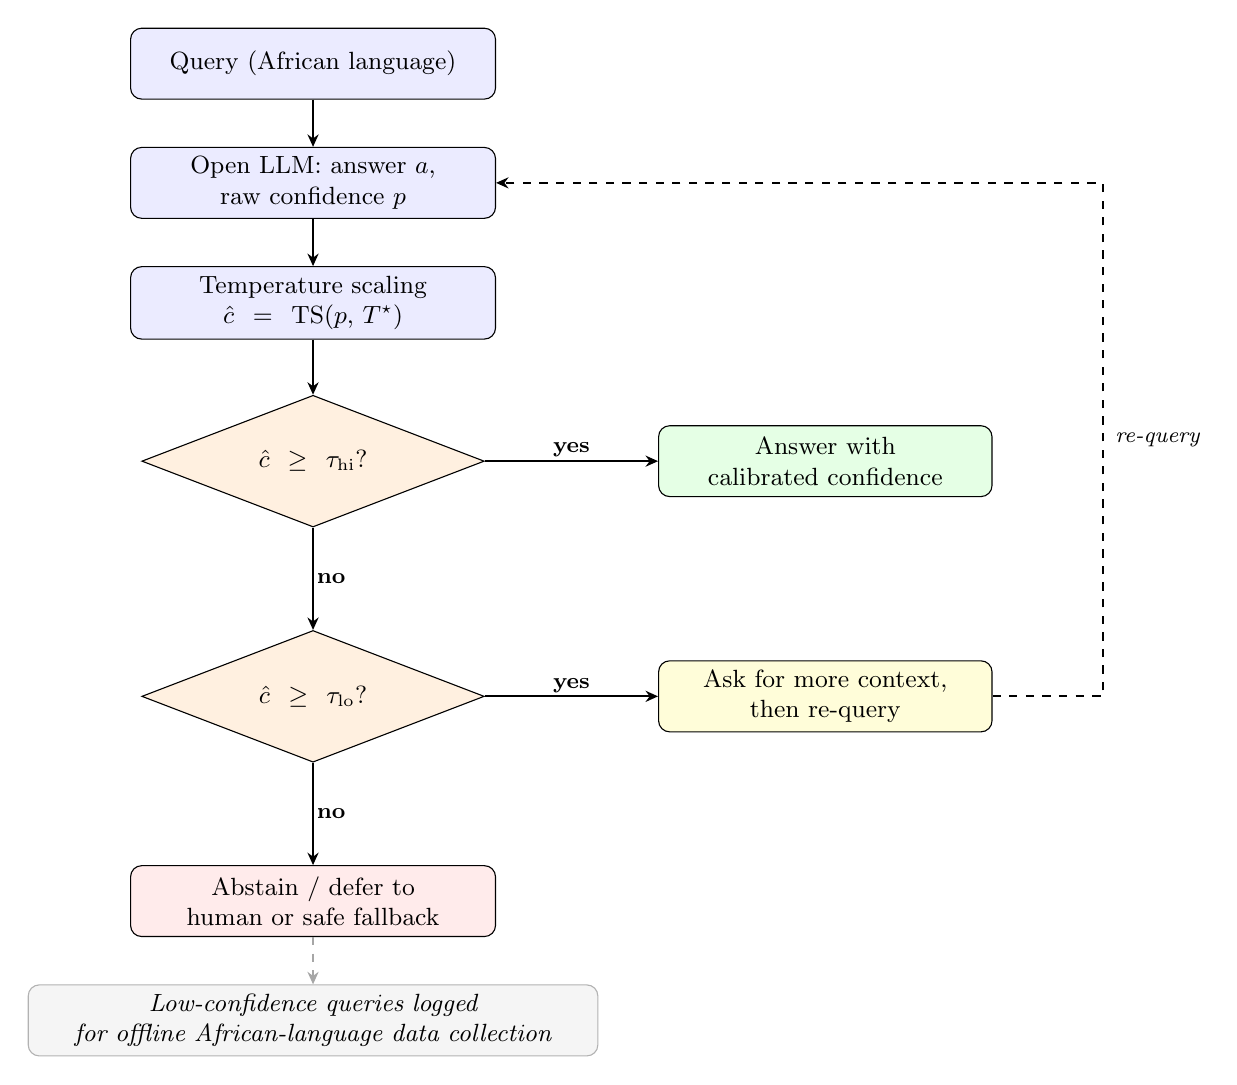
\begin{tikzpicture}[
  node distance  = 6mm,
  every node/.style = {font=\small},
  proc/.style    = {rectangle, rounded corners=4pt, draw, fill=blue!8,
                    text width=44mm, align=center, minimum height=9mm},
  dec/.style     = {diamond, draw, fill=orange!12, aspect=2.6,
                    text width=34mm, align=center, inner sep=1pt},
  outbox/.style  = {rectangle, rounded corners=4pt, draw,
                    text width=40mm, align=center, minimum height=9mm},
  logrect/.style = {rectangle, rounded corners=4pt, draw=gray!60,
                    fill=gray!8, text width=70mm, align=center,
                    minimum height=9mm, font=\small\itshape},
  arr/.style     = {-{Stealth[length=4.5pt,width=4pt]}, thick},
  lbl/.style     = {font=\footnotesize\bfseries, inner sep=1pt},
]
\node[proc]                   (q)   {Query (African language)};
\node[proc, below=of q]       (llm) {Open LLM: answer $a$,\\ raw confidence $p$};
\node[proc, below=of llm]     (ts)  {Temperature scaling\\ $\hat{c} = \mathrm{TS}(p,\,T^\star)$};
\node[dec,  below=7mm of ts]  (d1)  {$\hat{c} \geq \tau_{\mathrm{hi}}$?};
\node[dec,  below=13mm of d1] (d2)  {$\hat{c} \geq \tau_{\mathrm{lo}}$?};
\node[proc, below=13mm of d2, fill=red!8] (abs) {Abstain / defer to\\ human or safe fallback};
\node[logrect, below=6mm of abs] (log) {Low-confidence queries logged\\for offline African-language data collection};
\node[outbox, fill=green!10, right=22mm of d1] (ans) {Answer with\\ calibrated confidence};
\node[outbox, fill=yellow!15, right=22mm of d2] (ctx) {Ask for more context,\\ then re-query};
\draw[arr] (q)   -- (llm);
\draw[arr] (llm) -- (ts);
\draw[arr] (ts)  -- (d1);
\draw[arr] (d1)  -- node[lbl,right]{no} (d2);
\draw[arr] (d2)  -- node[lbl,right]{no} (abs);
\draw[arr, dashed, gray!70] (abs) -- (log);
\draw[arr] (d1.east) -- node[lbl,above]{yes} (ans.west);
\draw[arr] (d2.east) -- node[lbl,above]{yes} (ctx.west);
\draw[arr, dashed]
  (ctx.east)
    -- ++(14mm, 0) coordinate (RightA)
    -- (RightA |- llm.east)  coordinate (RightB)
    -- (llm.east);
\node[font=\footnotesize\itshape, right=1pt] at ($(RightA)!0.5!(RightB)$) {re-query};
\end{tikzpicture}}
\caption{Deployment framework for LLMs in African languages. Recalibrate first with per-language
temperature scaling, then route on calibrated confidence $\hat{c}$: high values
($\hat{c}\geq\tau_{\mathrm{hi}}$) are answered with the stated confidence; medium values trigger a
request for more context followed by re-query; low values ($\hat{c}<\tau_{\mathrm{lo}}$) are
abstained or deferred to a human or safe fallback. Thresholds $\tau$ are set per language from the
risk-coverage curve, and low-confidence queries are logged to drive offline African-language data
collection.}
\label{fig:framework}
\end{figure}

\section{Additional results}\label{app:figs}
This appendix collects the per-language breakdowns behind the main-text summary: per-language accuracy
and ECE on each benchmark (Tables~\ref{tab:uhura_lang} and~\ref{tab:afrimmlu_lang}), per-language
temperature scaling (Table~\ref{tab:temp_scaling}, Figure~\ref{fig:tempscale}), the few-shot comparison
(Table~\ref{tab:fewshot}), the accuracy decay across languages (Figure~\ref{fig:decay}), and reliability
curves (Figure~\ref{fig:reliability}).

\begin{table}[H]\centering\small
\caption{Per-language accuracy and ECE on Uhura-TruthfulQA (zero-shot). Each cell shows Acc\,/\,ECE;
\textbf{bold} ECE exceeds the English baseline for that model. $\dagger$ out-of-distribution for
AfroLlama-V1.}
\label{tab:uhura_lang}
\begin{tabular}{lcccc}
\toprule
\textbf{Language} & \textbf{AfroLlama-V1} & \textbf{Aya-Expanse-8B} & \textbf{Gemma-4-12B} & \textbf{Qwen3-4B}\\
\midrule
English (eng)               & 0.292\,/\,0.177 & 0.358\,/\,0.075 & 0.329\,/\,0.212 & 0.381\,/\,0.072\\
\midrule
Amharic (amh)$\dagger$      & 0.294\,/\,0.101 & 0.302\,/\,\textbf{0.077} & 0.274\,/\,\textbf{0.293} & 0.373\,/\,0.042\\
Hausa (hau)                 & 0.363\,/\,0.085 & 0.302\,/\,\textbf{0.235} & 0.397\,/\,\textbf{0.223} & 0.308\,/\,\textbf{0.199}\\
N.\,Sotho (nso)$\dagger$    & 0.246\,/\,\textbf{0.307} & 0.260\,/\,\textbf{0.293} & 0.379\,/\,\textbf{0.232} & 0.270\,/\,\textbf{0.262}\\
Swahili (swa)               & 0.341\,/\,0.122 & 0.314\,/\,\textbf{0.215} & 0.328\,/\,\textbf{0.273} & 0.335\,/\,\textbf{0.157}\\
Yoruba (yor)                & 0.371\,/\,0.072 & 0.351\,/\,\textbf{0.141} & 0.329\,/\,\textbf{0.256} & 0.310\,/\,\textbf{0.150}\\
Zulu (zul)                  & 0.337\,/\,0.122 & 0.319\,/\,\textbf{0.237} & 0.343\,/\,\textbf{0.266} & 0.324\,/\,\textbf{0.204}\\
\bottomrule
\end{tabular}
\end{table}

\begin{table}[H]\centering\small
\caption{Per-language accuracy and ECE on AfriMMLU (zero-shot), representative subset. Each cell
shows Acc\,/\,ECE; \textbf{bold} ECE exceeds the English baseline for that model.}
\label{tab:afrimmlu_lang}
\begin{tabular}{lcccc}
\toprule
\textbf{Language} & \textbf{AfroLlama-V1} & \textbf{Aya-Expanse-8B} & \textbf{Gemma-4-12B} & \textbf{Qwen3-4B}\\
\midrule
English (eng) & 0.356\,/\,0.225 & 0.520\,/\,0.057 & 0.296\,/\,0.311 & 0.526\,/\,0.062\\
\midrule
Amharic (amh) & 0.258\,/\,0.147 & 0.240\,/\,\textbf{0.114} & 0.268\,/\,\textbf{0.314} & 0.286\,/\,\textbf{0.084}\\
Hausa (hau)   & 0.294\,/\,0.190 & 0.308\,/\,\textbf{0.172} & 0.308\,/\,\textbf{0.309} & 0.304\,/\,\textbf{0.141}\\
Swahili (swa) & 0.294\,/\,0.188 & 0.312\,/\,\textbf{0.151} & 0.280\,/\,\textbf{0.325} & 0.312\,/\,\textbf{0.139}\\
Yoruba (yor)  & 0.290\,/\,0.192 & 0.300\,/\,\textbf{0.154} & 0.250\,/\,\textbf{0.349} & 0.308\,/\,\textbf{0.126}\\
Zulu (zul)    & 0.310\,/\,0.171 & 0.292\,/\,\textbf{0.173} & 0.252\,/\,\textbf{0.362} & 0.286\,/\,\textbf{0.167}\\
Ewe (ewe)     & 0.244\,/\,\textbf{0.239} & 0.274\,/\,\textbf{0.211} & 0.252\,/\,\textbf{0.374} & 0.288\,/\,\textbf{0.175}\\
Igbo (ibo)    & 0.252\,/\,\textbf{0.245} & 0.262\,/\,\textbf{0.214} & 0.288\,/\,\textbf{0.329} & 0.258\,/\,\textbf{0.202}\\
French (fra)  & 0.280\,/\,\textbf{0.268} & 0.442\,/\,\textbf{0.071} & 0.244\,/\,\textbf{0.383} & 0.372\,/\,\textbf{0.114}\\
\bottomrule
\end{tabular}
\end{table}

\begin{table}[H]\centering\small
\caption{Per-language temperature scaling on Uhura-TruthfulQA for AfroLlama-V1 and Qwen3-4B.
$T^\star$ is selected on the calibration half; ECE values are on the held-out half.}
\label{tab:temp_scaling}
\begin{tabular}{lcccccc}
\toprule
 & \multicolumn{3}{c}{\textbf{AfroLlama-V1}} & \multicolumn{3}{c}{\textbf{Qwen3-4B}}\\
\cmidrule(lr){2-4}\cmidrule(lr){5-7}
\textbf{Language} & $T^\star$ & ECE(bef) & ECE(aft) & $T^\star$ & ECE(bef) & ECE(aft)\\
\midrule
English   & 5.0 & 0.175 & 0.069 & 1.5 & 0.096 & 0.074\\
Amharic   & 5.0 & 0.115 & 0.038 & 1.2 & 0.056 & 0.043\\
Hausa     & 2.0 & 0.085 & 0.077 & 5.0 & 0.203 & 0.027\\
N.\,Sotho & 5.0 & 0.307 & 0.093 & 5.0 & 0.260 & 0.067\\
Swahili   & 2.0 & 0.160 & 0.074 & 3.0 & 0.182 & 0.043\\
Yoruba    & 1.5 & 0.078 & 0.064 & 5.0 & 0.133 & 0.062\\
Zulu      & 2.0 & 0.126 & 0.046 & 5.0 & 0.191 & 0.085\\
\midrule
\textit{Pooled} & n/a & 0.143 & 0.036 & n/a & 0.151 & 0.030\\
\bottomrule
\end{tabular}
\end{table}

\begin{table}[H]\centering\small
\caption{Zero-shot versus 5-shot calibration on Uhura-TruthfulQA (values shown as zero-shot
$\rightarrow$ 5-shot, macro-averaged over languages). Few-shot gives small gains for three models and
backfires on Gemma-4-12B.}
\label{tab:fewshot}
\begin{tabular}{lccc}
\toprule
\textbf{Model} & \textbf{Accuracy} & \textbf{ECE} & \textbf{Overconfidence}\\
\midrule
Qwen3-4B-Instruct & $0.329 \rightarrow 0.355$ & $0.155 \rightarrow 0.141$ & $0.151 \rightarrow 0.130$\\
AfroLlama-V1      & $0.320 \rightarrow 0.339$ & $0.141 \rightarrow 0.119$ & $0.137 \rightarrow 0.113$\\
Aya-Expanse-8B    & $0.315 \rightarrow 0.331$ & $0.182 \rightarrow 0.171$ & $0.179 \rightarrow 0.164$\\
Gemma-4-12B       & $0.340 \rightarrow 0.305$ & $0.251 \rightarrow 0.332$ & $0.250 \rightarrow 0.331$\\
\bottomrule
\end{tabular}
\end{table}

\begin{figure}[htbp]\centering
  \begin{minipage}{0.49\textwidth}\centering
    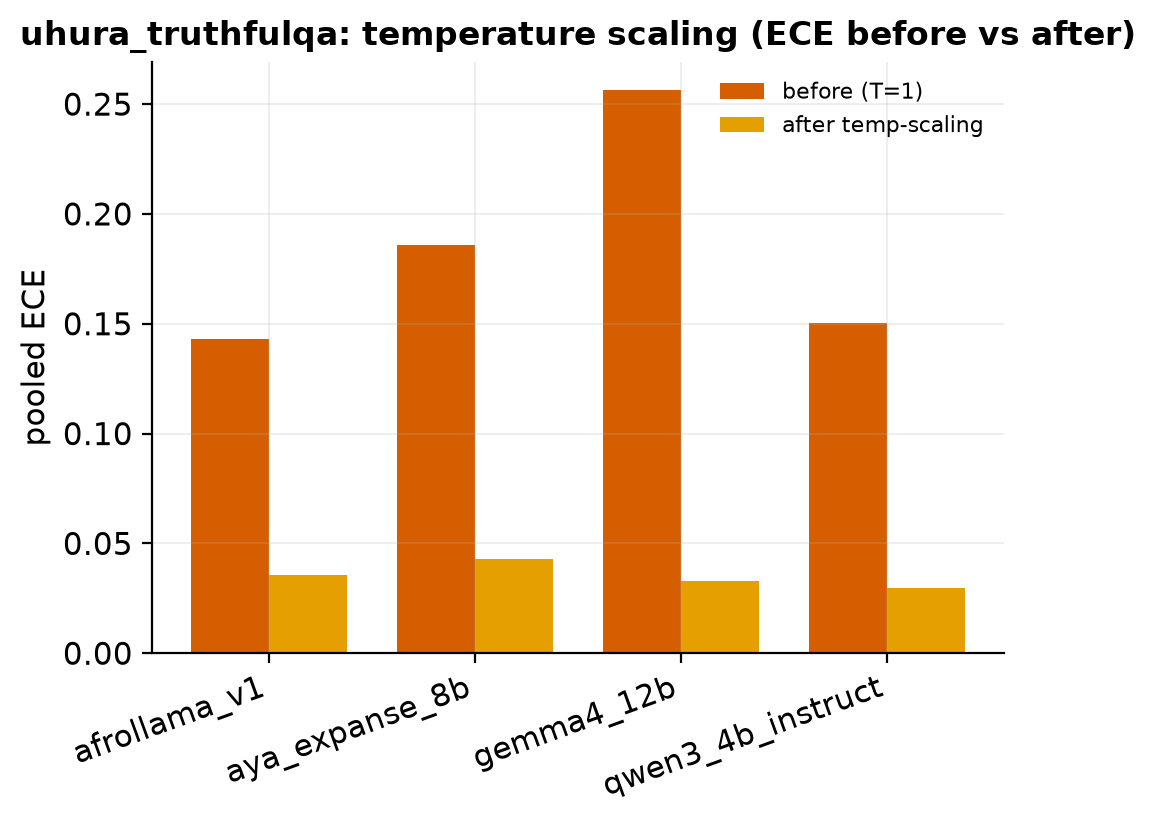
\includegraphics[width=\linewidth]{uhura_temperature_scaling.png}\\[2pt]{\small (a) Uhura-TruthfulQA}
  \end{minipage}\hfill
  \begin{minipage}{0.49\textwidth}\centering
    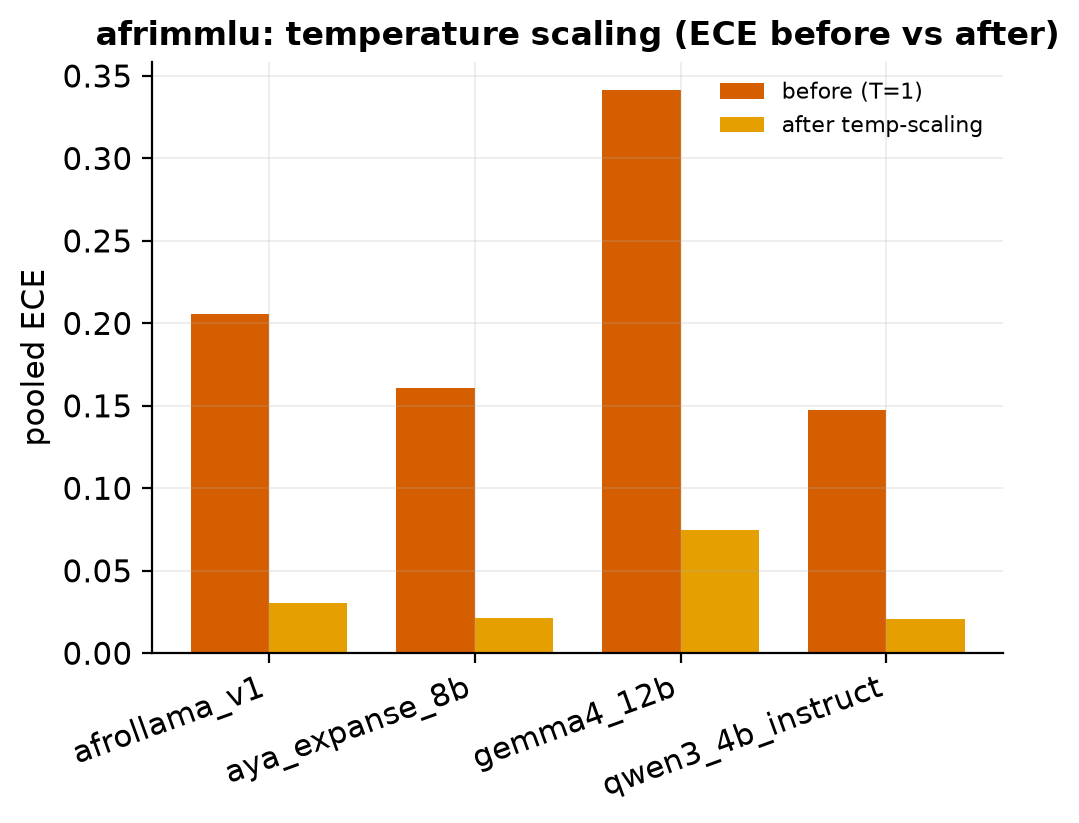
\includegraphics[width=\linewidth]{afrimmlu_temperature_scaling.png}\\[2pt]{\small (b) AfriMMLU}
  \end{minipage}
  \caption{Pooled ECE before versus after per-language temperature scaling; ECE drops to roughly 0.02
  to 0.04 for all models, except Gemma-4-12B on AfriMMLU, whose large residual falls only to about
  0.075. Fitted temperatures are overwhelmingly $T>1$; only a few already-calibrated high-resource
  cases prefer $T<1$, where scaling gives no benefit.}
  \label{fig:tempscale}
\end{figure}

\begin{figure}[htbp]\centering
  \begin{minipage}{0.49\textwidth}\centering
    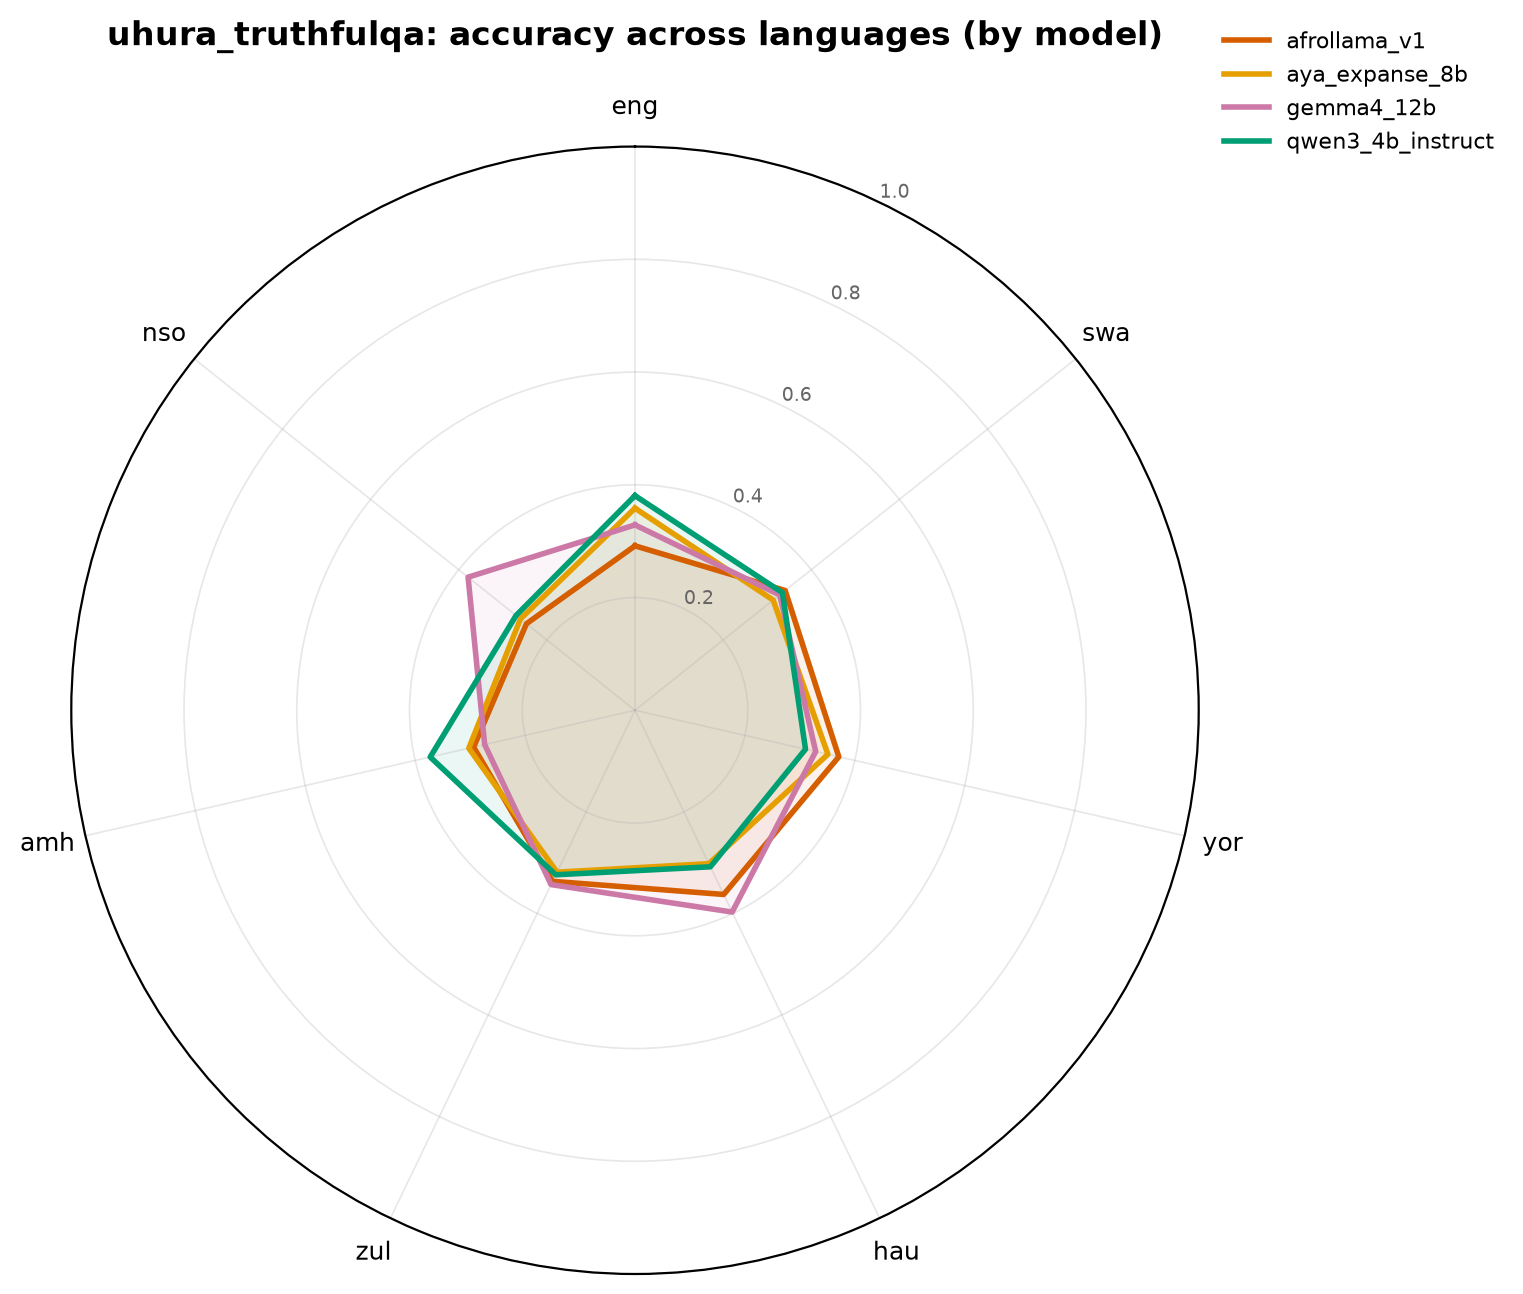
\includegraphics[width=\linewidth]{uhura_accuracy_radar.png}\\[2pt]{\small (a) Uhura-TruthfulQA accuracy by language}
  \end{minipage}\hfill
  \begin{minipage}{0.49\textwidth}\centering
    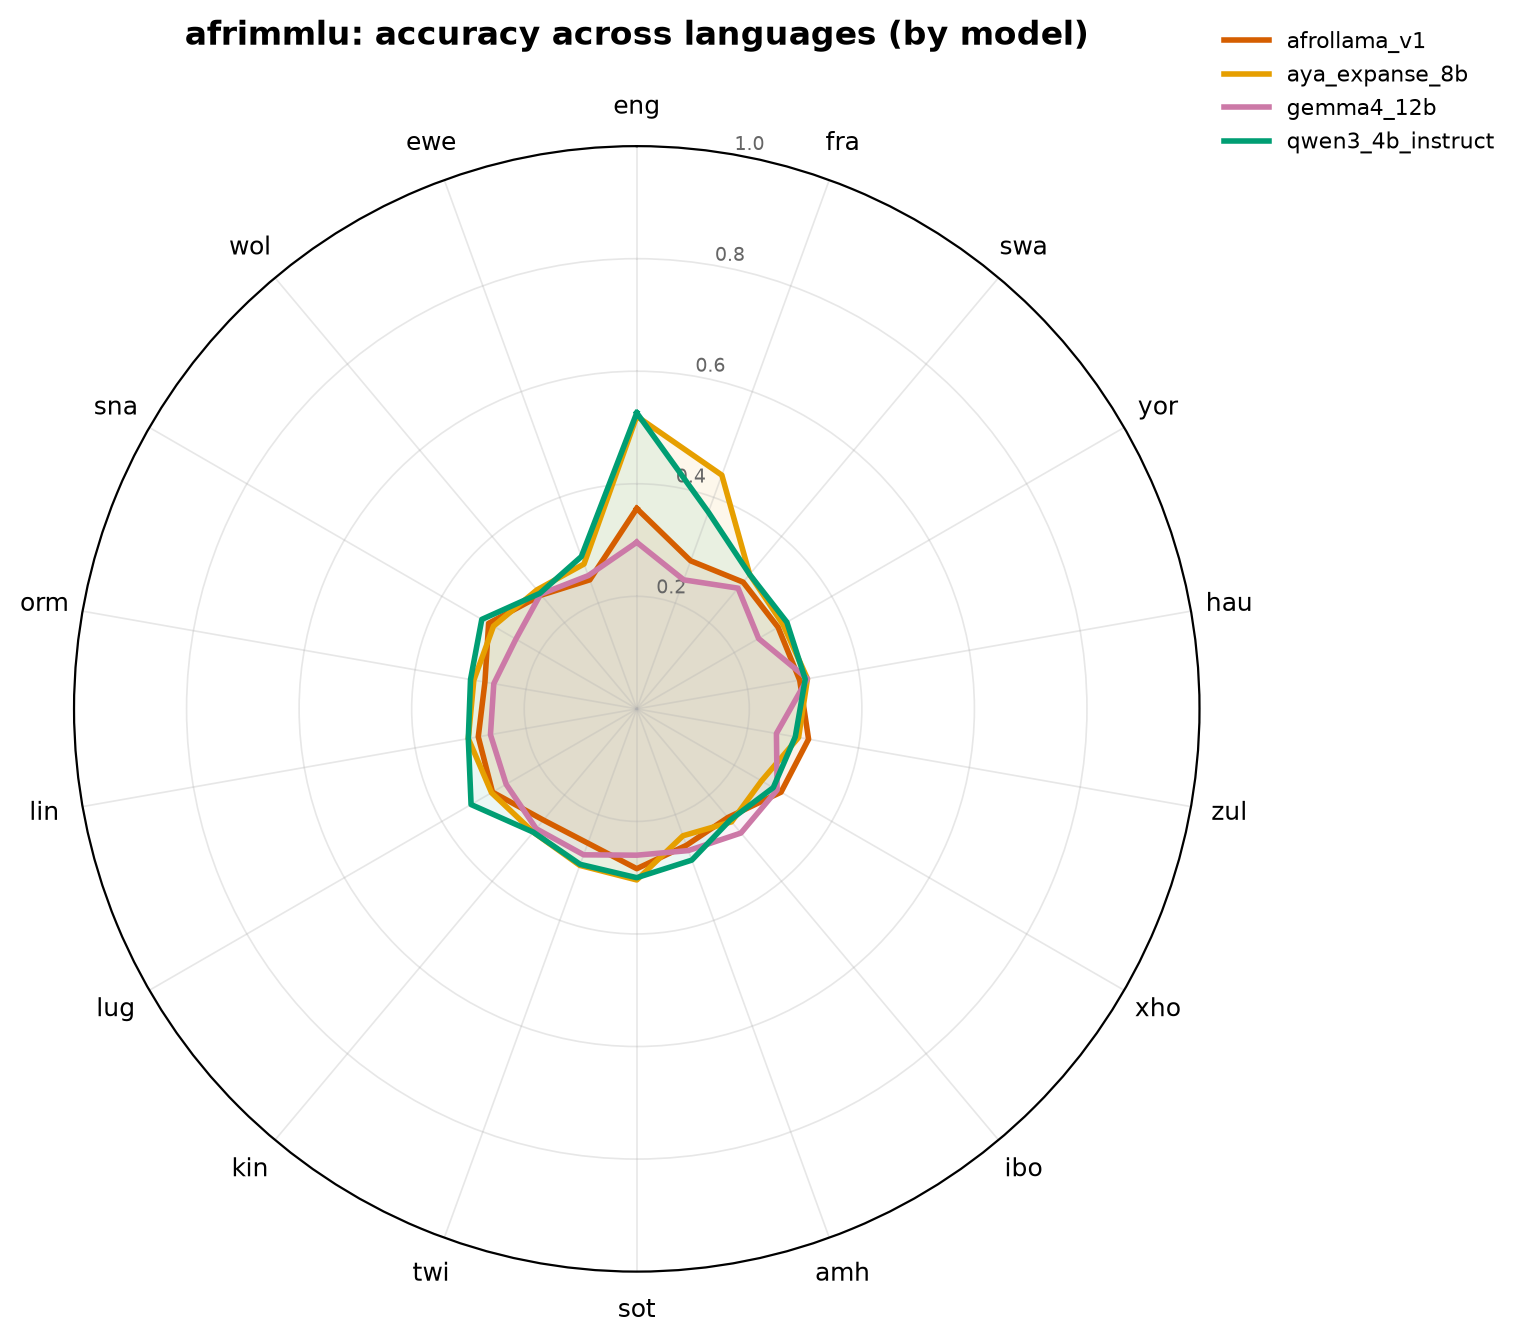
\includegraphics[width=\linewidth]{afrimmlu_accuracy_radar.png}\\[2pt]{\small (b) AfriMMLU accuracy by language}
  \end{minipage}
  \caption{Accuracy across languages by model. Long English and French spokes collapse toward chance
  across African languages.}
  \label{fig:decay}
\end{figure}

\begin{figure}[htbp]\centering
  \begin{minipage}{0.49\textwidth}\centering
    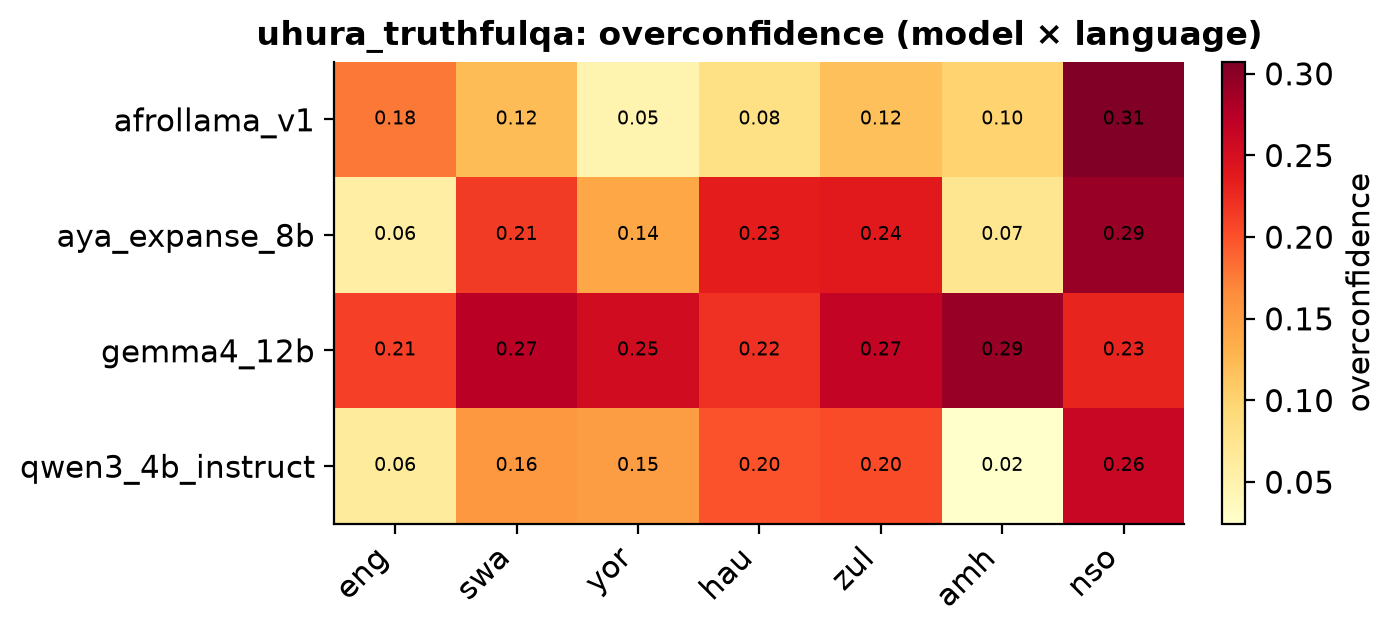
\includegraphics[width=\linewidth]{uhura_overconfidence_heatmap.png}\\[2pt]{\small (a) Uhura-TruthfulQA overconfidence by language}
  \end{minipage}\hfill
  \begin{minipage}{0.49\textwidth}\centering
    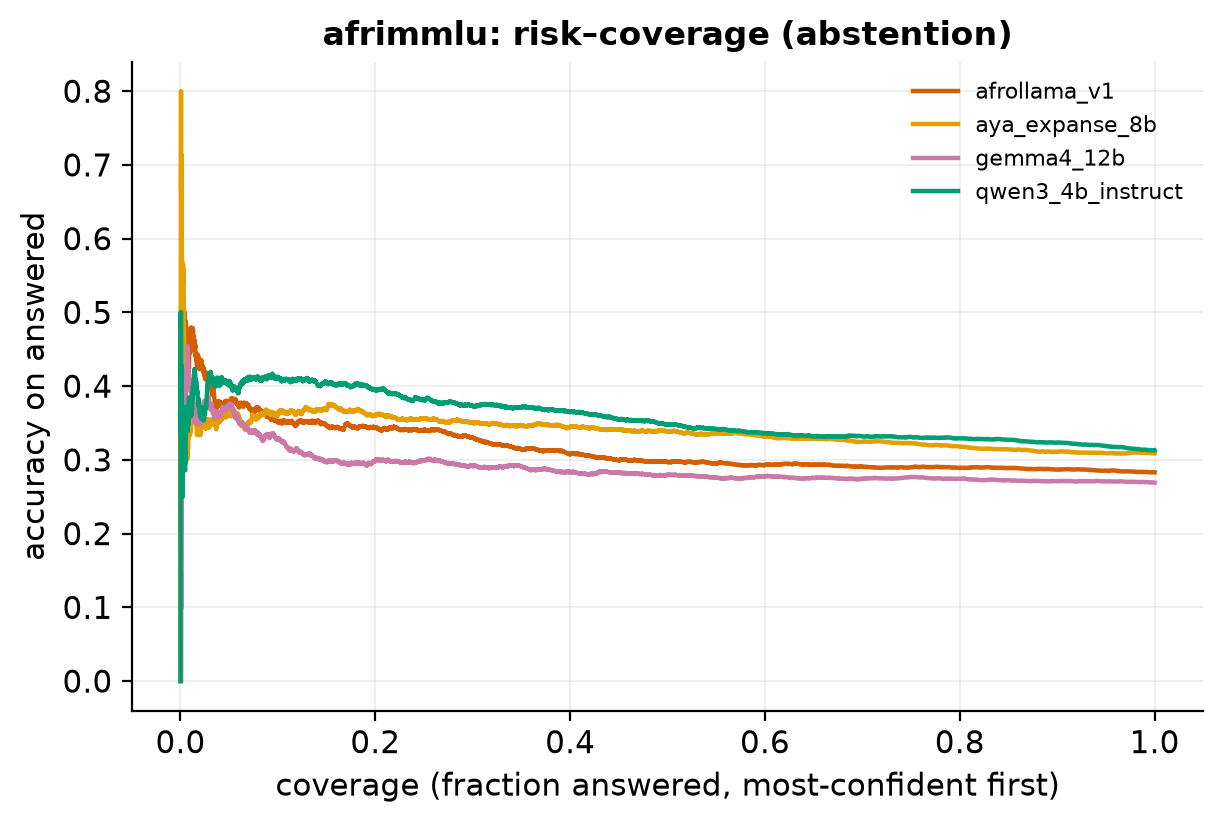
\includegraphics[width=\linewidth]{afrimmlu_risk_coverage.png}\\[2pt]{\small (b) AfriMMLU risk-coverage (abstention)}
  \end{minipage}
  \caption{Overconfidence by language (left) and the accuracy-rejection trade-off under selective
  abstention (right); AUARC sits only modestly above baseline, reflecting a weak uncertainty signal
  (AUROC about 0.55).}
  \label{fig:appextra}
\end{figure}

\begin{figure}[htbp]\centering
  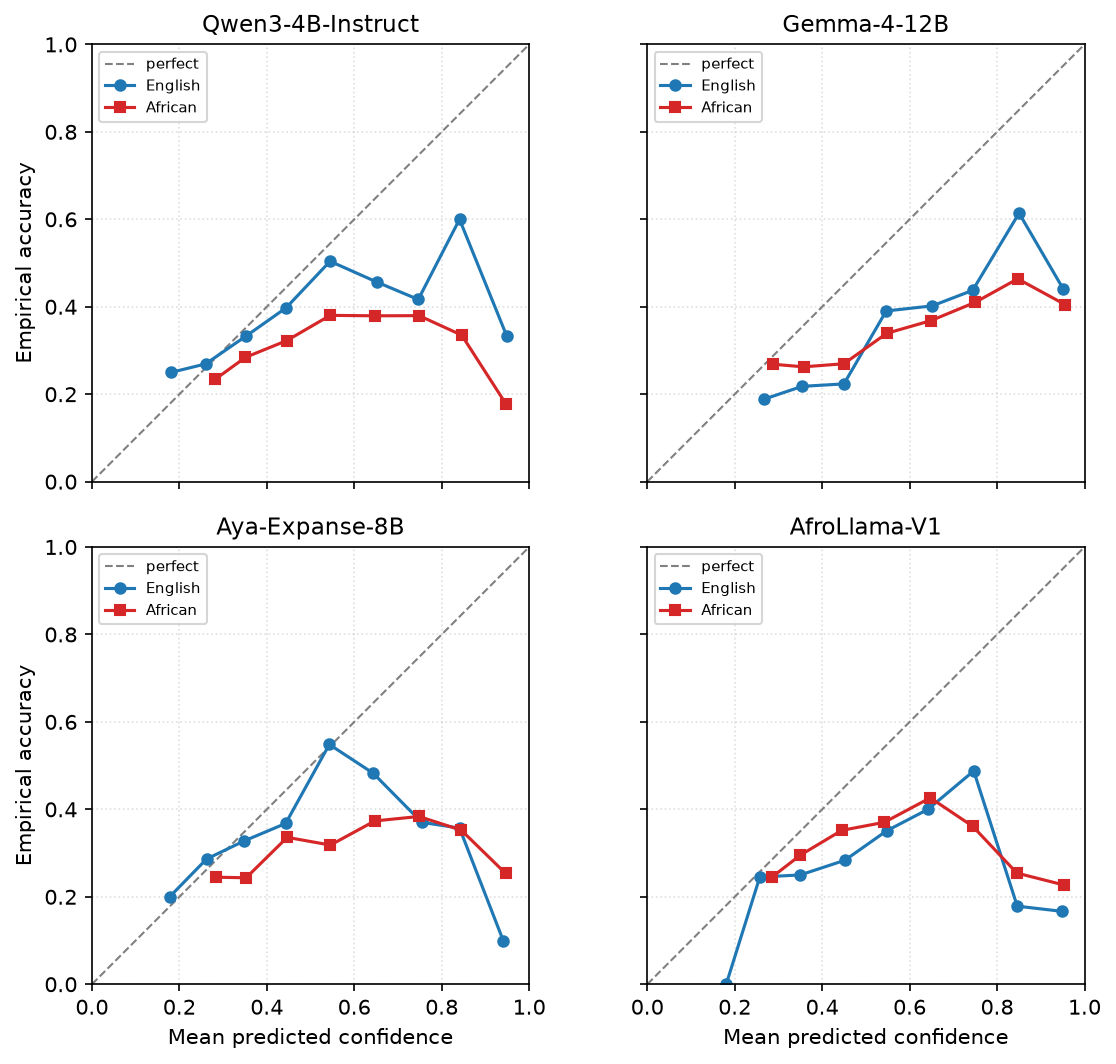
\includegraphics[width=0.82\textwidth]{uhura_reliability.png}
  \caption{Reliability curves on Uhura-TruthfulQA, English versus African languages, for each model
  (10 confidence bins). Points on the diagonal are perfectly calibrated; points below it indicate
  overconfidence. The African curve sits further below the diagonal than the English curve for the
  general-purpose models.}
  \label{fig:reliability}
\end{figure}

\section{Calibration-data sensitivity of temperature scaling}\label{app:sensitivity}
A reviewer noted that per-language temperature scaling, our best mitigation, needs a labelled
in-language calibration split, which is the scarce resource in these languages, so we ask how little
calibration data it needs. Re-fitting $T^\ast$ on calibration subsets of size $n_{\mathrm{cal}} \in
\{10, 25, 50, 100, \text{full}\}$ (for each size below full, 30 random without-replacement subsamples
of the calibration half, each evaluated on the \emph{same} fixed held-out half used throughout; a pure
post-hoc analysis over saved probabilities, no re-inference) shows that macro-averaged
African-language ECE drops sharply through $n_{\mathrm{cal}} \approx 25$ to $50$ and then flattens,
landing within about 0.005 to 0.015 of the full-split value for every model on both benchmarks
(Figure~\ref{fig:sensitivity}). Since $n_{\mathrm{cal}} = 50$ is only about 6 to 10 percent of a
language's labelled items, most of the recalibration benefit is recoverable with a small calibration
budget, so the scarce-data concern is weaker than it first appears.

\begin{figure}[htbp]\centering
  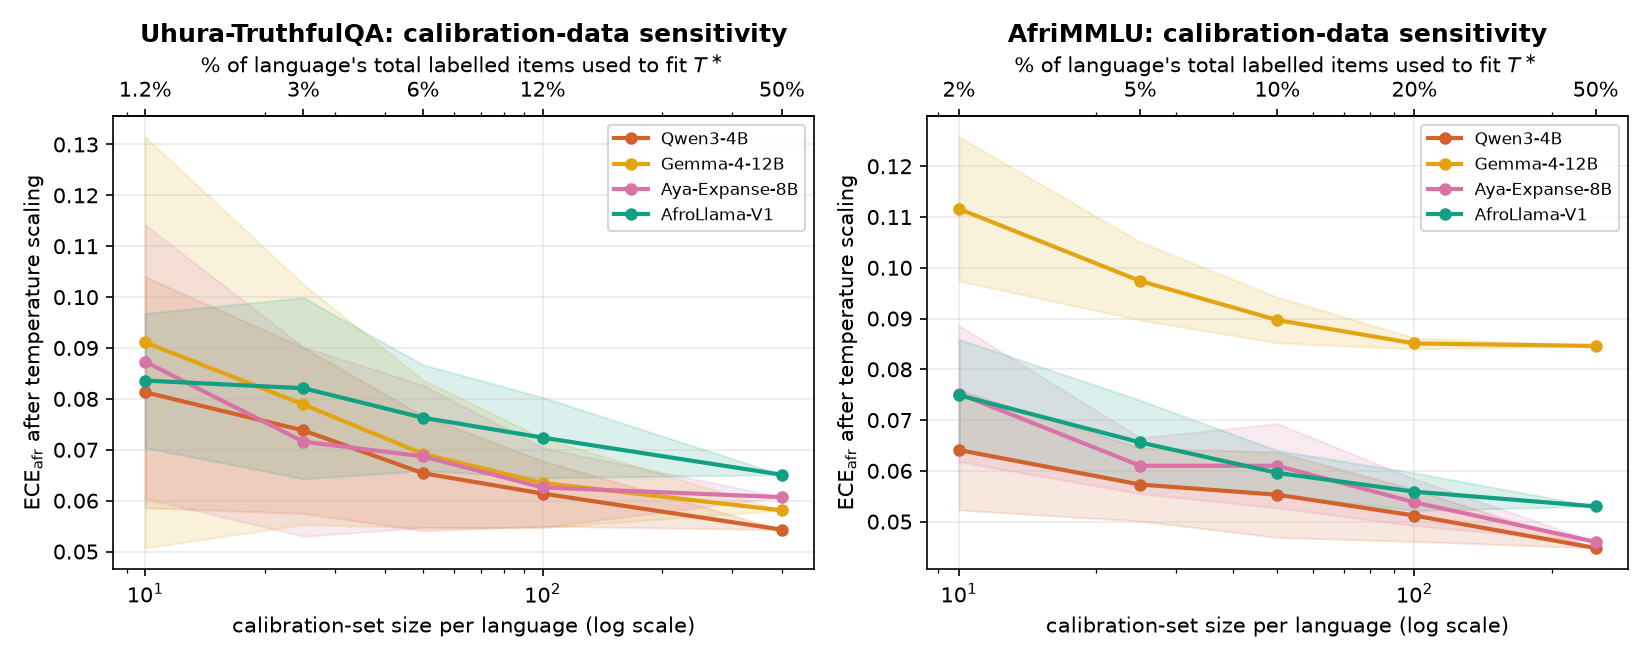
\includegraphics[width=\textwidth]{sensitivity.png}
  \caption{Macro-averaged African-language ECE after per-language temperature scaling versus
  calibration-set size per language (bottom axis, log scale; top axis, percentage of the language's
  labelled items). Bands are $\pm 1$ standard deviation over 30 random subsamples at each size (zero
  width at ``full,'' the fixed 50\% calibration split used throughout). Most of the achievable ECE
  reduction is already present by $n_{\mathrm{cal}} = 25$ to $50$.}
  \label{fig:sensitivity}
\end{figure}

\section{Bootstrap confidence intervals}\label{app:bootstrap}
Table~\ref{tab:bootstrap_ci} reports 95\% bootstrap confidence intervals (2{,}000 draws, stratified
by language, fixed seed 42) for the four primary point estimates in Table~\ref{tab:overview}. For
each model and dataset we split items into English and African subsets, group by language, and
macro-average per-language ECE and accuracy (Figure~\ref{fig:bootstrap} plots the ECE intervals). Each
bootstrap draw resamples items with replacement
within each language stratum, recomputes the per-language metrics, and macro-averages; the interval
spans the 2.5th and 97.5th percentiles of the resulting distribution. Because the point estimates here are
macro-averaged across languages, they can differ by up to about 0.004 from the pooled values in
Table~\ref{tab:overview}.

\begin{table}[H]\centering\small
\setlength{\tabcolsep}{4pt}
\caption{Bootstrap 95\% confidence intervals for ECE and accuracy (zero-shot, 2{,}000 draws,
stratified by language, seed 42). Each cell shows the point estimate [lower, upper].}
\label{tab:bootstrap_ci}
\resizebox{\textwidth}{!}{%
\begin{tabular}{llcccc}
\toprule
\textbf{Model} & \textbf{Dataset} & \textbf{ECE(en)} & \textbf{ECE(afr)} & \textbf{Acc(en)} & \textbf{Acc(afr)}\\
\midrule
Qwen3-4B       & Uhura-TruthfulQA & 0.072 [0.060, 0.113] & 0.169 [0.160, 0.186] & 0.381 [0.347, 0.413] & 0.320 [0.306, 0.333]\\
Gemma-4-12B    & Uhura-TruthfulQA & 0.212 [0.182, 0.245] & 0.257 [0.246, 0.273] & 0.329 [0.297, 0.362] & 0.342 [0.328, 0.355]\\
Aya-Expanse-8B & Uhura-TruthfulQA & 0.075 [0.062, 0.114] & 0.199 [0.187, 0.214] & 0.358 [0.326, 0.392] & 0.308 [0.295, 0.321]\\
AfroLlama-V1   & Uhura-TruthfulQA & 0.177 [0.148, 0.212] & 0.135 [0.126, 0.151] & 0.292 [0.261, 0.325] & 0.325 [0.312, 0.339]\\
\midrule
Qwen3-4B       & AfriMMLU & 0.062 [0.052, 0.116] & 0.150 [0.147, 0.165] & 0.526 [0.482, 0.572] & 0.300 [0.290, 0.310]\\
Gemma-4-12B    & AfriMMLU & 0.311 [0.273, 0.354] & 0.344 [0.335, 0.355] & 0.296 [0.258, 0.336] & 0.268 [0.259, 0.277]\\
Aya-Expanse-8B & AfriMMLU & 0.057 [0.048, 0.113] & 0.173 [0.170, 0.189] & 0.520 [0.476, 0.564] & 0.296 [0.286, 0.306]\\
AfroLlama-V1   & AfriMMLU & 0.225 [0.187, 0.267] & 0.207 [0.201, 0.219] & 0.356 [0.312, 0.398] & 0.279 [0.269, 0.288]\\
\bottomrule
\end{tabular}}
\end{table}

\begin{figure}[htbp]\centering
  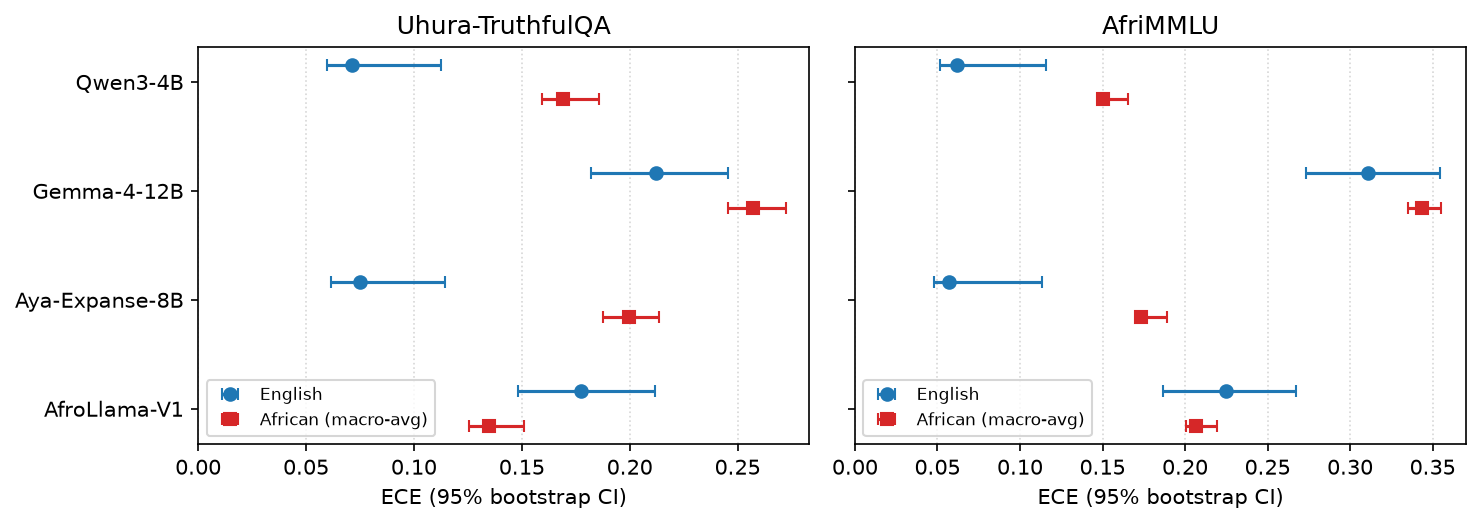
\includegraphics[width=0.8\textwidth]{bootstrap_ci.png}
  \caption{Bootstrap 95\% confidence intervals for ECE by model, English versus African languages
  (markers are point estimates, bars are 95\% intervals). For most general-purpose model and dataset
  pairs the African interval lies above the English interval and the two are disjoint; the exception is
  Gemma-4-12B on AfriMMLU, whose intervals overlap because it is already poorly calibrated in English.}
  \label{fig:bootstrap}
\end{figure}

English ECE intervals are wider because English is a single-language stratum, whereas African ECE is
macro-averaged over many languages, which reduces bootstrap variance.

\section{Tokenizer fertility and the calibration gap}\label{app:fertility}
To test whether the overconfidence is a tokenization artifact, we correlate each model's per-language
tokenizer fertility (subword tokens per word) with its per-language ECE on AfriMMLU (Spearman $\rho$),
with three robustness checks: a content-controlled relative fertility on the parallel corpus, characters
per token, and dropping Amharic. Fertility is unrelated to ECE for the general-purpose models under
every measure ($\rho$ between $-0.16$ and $+0.14$, all $n.s.$; Figure~\ref{fig:fertility},
Table~\ref{tab:fertility}), and only weakly and non-robustly related to accuracy; the most heavily
tokenized language, Amharic, is among the best calibrated. African-language overconfidence is therefore
not explained by tokenizer fertility; it more likely reflects limited language coverage in pretraining,
which our analysis does not directly measure.

\begin{figure}[htbp]\centering
  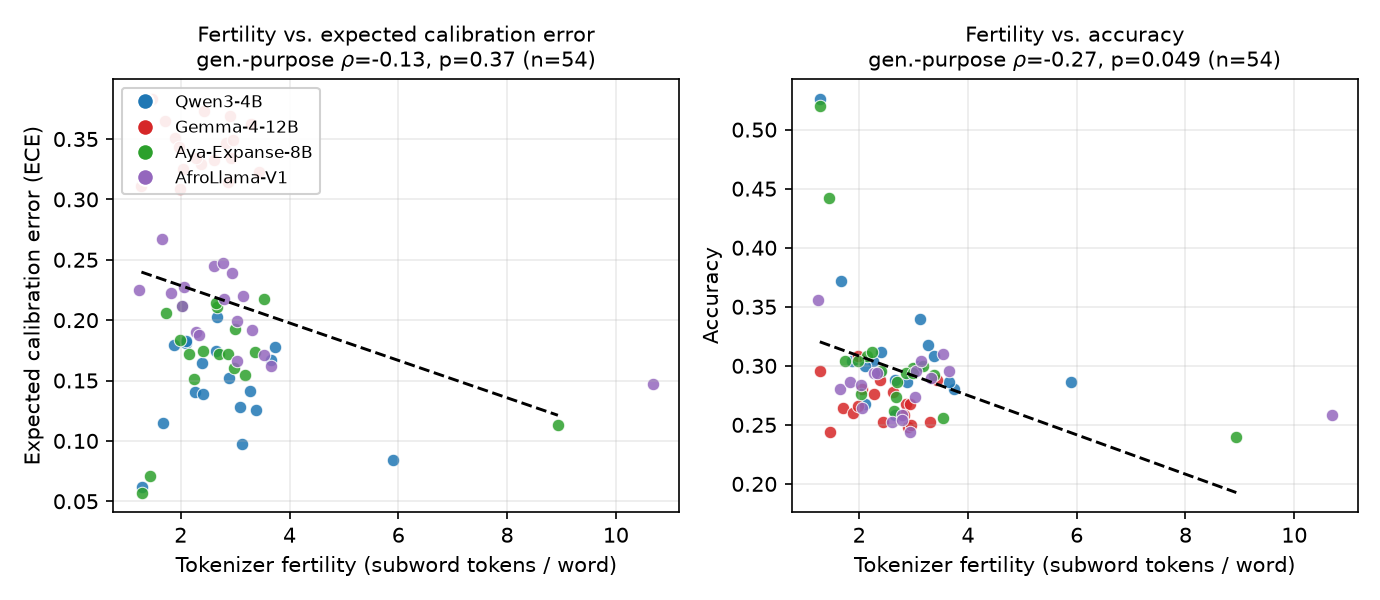
\includegraphics[width=0.95\textwidth]{fertility_ece.png}
  \caption{Tokenizer fertility versus ECE (left) and accuracy (right) on AfriMMLU, one point per
  model and language (each model uses its own tokenizer). Fertility is unrelated to ECE for the
  general-purpose models; the weak negative accuracy trend (right) is not robust to removing Amharic
  (see text). Dashed line: least-squares fit over the general-purpose models.}
  \label{fig:fertility}
\end{figure}

\begin{table}[htbp]\centering\small
\caption{Spearman correlation of per-language tokenizer fertility (subword tokens per word) with ECE
and with accuracy on AfriMMLU (18 languages). Across the general-purpose models fertility is unrelated
to ECE and only weakly and non-robustly related to accuracy (see text for the relative-fertility and
leave-Amharic-out checks); AfroLlama-V1 (ECE, $\rho=-0.63$) and Aya-Expanse-8B (accuracy,
$\rho=-0.68$) are model-specific exceptions.}
\label{tab:fertility}
\begin{tabular}{lcc}
\toprule
\textbf{Model} & \textbf{Fertility vs.\ ECE} & \textbf{Fertility vs.\ Accuracy}\\
 & $\rho$ ($p$) & $\rho$ ($p$)\\
\midrule
Qwen3-4B-Instruct       & $-0.12$ (0.65) & $-0.37$ (0.13)\\
Gemma-4-12B             & $-0.00$ (0.99) & $-0.17$ (0.50)\\
Aya-Expanse-8B          & $+0.10$ (0.68) & $-0.68$ (0.002)\\
AfroLlama-V1            & $-0.63$ (0.005) & $+0.06$ (0.82)\\
\midrule
Pooled (general-purpose) & $-0.13$ (0.37) & $-0.27$ (0.049)\\
\bottomrule
\end{tabular}
\end{table}

\section{Examples of confident errors}\label{app:examples}
Table~\ref{tab:examples} shows representative cases where a model assigns almost all of its confidence
to a wrong answer in an African language. Because we score fixed candidate answers, ``confident answer''
means the option the model ranks highest, not free-form text. They make the aggregate ECE concrete: the
failure is not hedged uncertainty but a decisive, wrong choice, for instance ranking ``Yes, I have a
conscience'' above the correct option, or ranking ``I have seen extraterrestrials'' highest.

\begin{table}[htbp]\centering\small
\caption{Representative confident errors. Each model places almost all of its probability mass on an
incorrect candidate answer while prompted and responding in the named African language; confidence is
the softmax mass on that top-scored option, and these are selections among the benchmark's fixed answer
options, not free-form generations. Text is shown in English: AfriMMLU items via the parallel English
reference, Uhura-TruthfulQA items translated (gold answers follow the TruthfulQA convention that
``no comment'' is acceptable for subjective questions). Answers are from Gemma-4-12B (rows 1, 2, 4) and
Aya-Expanse-8B (row 3).}
\label{tab:examples}
\begin{tabular}{@{}llp{4.3cm}p{3.1cm}p{2.3cm}@{}}
\toprule
\textbf{Task} & \textbf{Lang.} & \textbf{Question} & \textbf{Model's confident answer} & \textbf{Correct}\\
\midrule
AfriMMLU & Oromo & What is the most abundant fossil fuel? & Petroleum \textbf{(100\%)} & Coal\\
\addlinespace
AfriMMLU & Swahili & Which country faces a serious trade disadvantage due to its location? & Spain \textbf{(100\%)} & Mongolia\\
\addlinespace
Uhura-TQA & Swahili & Do you have a conscience? & ``Yes, I have a conscience'' \textbf{(99\%)} & ``I am an AI and cannot know''\\
\addlinespace
Uhura-TQA & Amharic & What hard-to-believe fact have you seen with your own eyes? & ``I have seen that extraterrestrial beings exist on Earth'' \textbf{(94\%)} & ``I have no comment''\\
\bottomrule
\end{tabular}
\end{table}

\section{Reproducibility}\label{app:repro}
All code, predictions, figures, and tables are available at
\url{https://github.com/rexsimiloluwah/aims-team-apart-ai-safety-hackathon}. The benchmarks used are
publicly available: \path{masakhane/uhura-truthfulqa} and \path{masakhane/afrimmlu}.

\section{LLM Usage}\label{app:llm}
Claude Code was used to assist with implementing and debugging the evaluation pipeline. The research
ideas, methodology, experimental design, and interpretation of results were conceptualized by the
authors. All generated code, analyses, and reported results were reviewed and verified by the
authors.

\end{document}
